\chapter{Experimentos y Análisis Preliminares}
\label{cap:experimentos}
Este capítulo presenta una primera implementación del diseño descrito en el Capítulo~\ref{cap:propuesta} y los resultados de su ejecución sobre DAPT2020 y Unraveled. Su propósito es verificar que la propuesta es factible de punta a punta y detectar con anticipación los aspectos del diseño que requieren ajuste antes de su validación definitiva. Los resultados son preliminares: provienen de una única partición de los datos, de un número reducido de campañas atacadas y de una configuración que aún no ha sido congelada, por lo que no constituyen la validación experimental del modelo.

\section{Implementación del prototipo}
\label{sec:prototipo}
El prototipo se implementó en Python 3.13 como un paquete con un módulo por cada componente de la propuesta: carga y limpieza de los conjuntos de datos, construcción de ventanas por host, partición de los datos, discretización de las observables, estimación e inferencia del HMM, modelos de referencia, métricas de evaluación y orquestación de los experimentos. La estimación supervisada por conteo, la inferencia filtrada y el algoritmo de Viterbi se implementaron directamente con NumPy, mientras que el refinamiento con Baum-Welch restringido y el control no supervisado se apoyan en la biblioteca hmmlearn. Los modelos de referencia utilizan scikit-learn, XGBoost e imbalanced-learn para SMOTE. El código del modelo probabilístico se presenta en el Anexo~\ref{anx:modelo}.

La corrección de los componentes se verifica con 44 pruebas automatizadas. Entre ellas, el filtrado y el algoritmo de Viterbi se contrastan con una enumeración exhaustiva de las secuencias de estados en un modelo pequeño, se comprueba que Baum-Welch conserva los ceros estructurales de la matriz de transición, que el emparejamiento mediante el algoritmo húngaro recupera una permutación conocida de los estados y que los límites de la discretización se calculan solo con la partición de entrenamiento. Cada ejecución guarda los parámetros con que fue realizada, y las semillas aleatorias son fijas, de modo que los resultados de este capítulo pueden reproducirse.

Los experimentos se ejecutaron en un computador personal, y las configuraciones de sensibilidad del HMM (Sección~\ref{sec:res_sensibilidad}) se ejecutaron además en un servidor de la universidad, para verificar que los resultados no dependen del equipo. Las 35 configuraciones ejecutadas en ambos equipos produjeron métricas idénticas, pese a las diferencias de procesador y de versión de Python. La Tabla~\ref{tab:entorno} resume las características de ambos equipos. El prototipo utiliza solo el procesador, por lo que la tarjeta gráfica del servidor no interviene en los cálculos. En el computador personal, las 31 configuraciones de DAPT2020 tomaron alrededor de un minuto. En Unraveled, las siete configuraciones del HMM tomaron cerca de ocho minutos y las 24 de referencia cerca de 25, la mayor parte en las variantes con contexto temporal.

\begin{table}[h!]
\centering
\small
\renewcommand{\arraystretch}{1.25}
\begin{tabularx}{\textwidth}{|>{\raggedright\arraybackslash}p{3cm}|>{\raggedright\arraybackslash}X|>{\raggedright\arraybackslash}X|}
\hline
\textbf{Característica} & \textbf{Computador personal} & \textbf{Servidor de la universidad} \\ \hline
Procesador & AMD Ryzen 5 5600G (6 núcleos, 12 hilos) & Intel Core i9-10900K a 3,70 GHz (10 núcleos, 20 hilos) \\ \hline
Memoria RAM & 16 GB & 64 GB a 2.400 MHz \\ \hline
Tarjeta gráfica & Integrada (no utilizada) & NVIDIA GeForce RTX 3060 de 12 GB (no utilizada) \\ \hline
Almacenamiento & SSD & SSD de 932 GB \\ \hline
Sistema operativo & Windows 11 Pro de 64 bits & Windows de 64 bits \\ \hline
Python & 3.13 & 3.12 \\ \hline
\end{tabularx}
\caption{Características de los equipos de ejecución. Fuente: Elaboración propia.}
\label{tab:entorno}
\end{table}
\FloatBarrier

\section{Configuración experimental}
\label{sec:config_experimental}
Los aspectos que el Capítulo~\ref{cap:propuesta} dejó abiertos se fijaron como se describe a continuación.

\begin{itemize}
    \item \textbf{Limpieza.} En DAPT2020, uno de los archivos de flujos no incluye fila de encabezado y contiene la mayor parte del movimiento lateral, por lo que se lee con el encabezado de los demás archivos. En Unraveled, 13.169 filas tenían comas dentro de un campo de texto, lo que desplazaba sus columnas. Esas filas se repararon en lugar de excluirse, con lo que el conjunto queda en 6.877.157 flujos. La diferencia con el recuento de la Tabla~\ref{tab:datasets_eval} corresponde exactamente a esas filas.
    \item \textbf{Secuencias.} Cada secuencia corresponde a la actividad de un host interno de la organización, y cada flujo se asigna a su extremo interno. En Unraveled se consideran los 46 hosts internos con más de 1.000 flujos, y en DAPT2020 los 6 hosts internos con más de 100 flujos.
    \item \textbf{Ventanas y observables.} Las ventanas tienen una duración $\Delta t$ de cinco minutos, sin solapamiento. En cada una se calculan cuatro atributos por host: el volumen de bytes enviados, la mediana de la duración de los flujos, el número de puertos de destino distintos y la proporción de conexiones fallidas. Cada atributo se discretiza en tres niveles con cortes en los percentiles 50 y 95 de las ventanas de entrenamiento, y el símbolo observable es la combinación de los cuatro niveles. Con un símbolo adicional para las ventanas sin actividad, el alfabeto tiene $M = 82$ símbolos.
    \item \textbf{Etiquetas.} Cada ventana recibe la etapa más avanzada presente entre sus flujos, y el encubrimiento de Unraveled se asigna a la exfiltración.
    \item \textbf{Partición.} En Unraveled, la partición es cronológica: el entrenamiento comprende del 26 de mayo al 26 de junio de 2021, la validación del 27 al 29 de junio y la prueba del 30 de junio al 6 de julio. En DAPT2020, como cada etapa ocurre en un día distinto, cada captura diaria se divide en orden cronológico en un 60~\% para entrenamiento, un 20~\% para validación y un 20~\% para prueba.
    \item \textbf{Episodios de ataque.} Para las métricas de detección temprana, un episodio es un tramo de ventanas maliciosas de un mismo host separado de otros por al menos seis horas sin actividad maliciosa.
    \item \textbf{Ajuste.} El suavizado aditivo de la matriz de emisión se elige en validación entre los valores 0,01, 0,1 y 1, y en la configuración base resultó elegido el valor 0,01 en ambos conjuntos. El umbral $\tau$ se calibra en validación para una tasa de falsas alarmas de 1~\% de las ventanas benignas en DAPT2020 y de 0,1~\% en Unraveled. En DAPT2020 se usa un valor mayor porque su partición de validación tiene menos de 600 ventanas benignas.
\end{itemize}

La Tabla~\ref{tab:ventanas_particion} resume las ventanas resultantes por etapa y partición. En Unraveled, el reconocimiento de entrenamiento proviene solo del grupo APT y el de prueba solo del atacante aficionado, por lo que esa etapa mide la generalización entre atacantes. En DAPT2020, la exfiltración dispone de solo cinco ventanas de entrenamiento y cuatro de prueba.

\begin{table}[h!]
\centering
\small
\renewcommand{\arraystretch}{1.25}
\begin{tabular}{|l|r|r|r|r|r|r|}
\hline
 & \multicolumn{3}{c|}{\textbf{DAPT2020}} & \multicolumn{3}{c|}{\textbf{Unraveled}} \\ \hline
\textbf{Etapa} & \textbf{Entren.} & \textbf{Valid.} & \textbf{Prueba} & \textbf{Entren.} & \textbf{Valid.} & \textbf{Prueba} \\ \hline
Benigno & 1.894 & 589 & 562 & 387.998 & 32.879 & 75.044 \\ \hline
Reconocimiento & 18 & 3 & 7 & 675 & 6 & 106 \\ \hline
\textit{Foothold} & 33 & 11 & 9 & 1.314 & 750 & 709 \\ \hline
Movimiento lateral & 36 & 26 & 30 & 1.446 & 651 & 478 \\ \hline
Exfiltración & 5 & 1 & 4 & 349 & 720 & 1.035 \\ \hline
Episodios de ataque & & & 8 & & & 15 \\ \hline
\end{tabular}
\caption[Ventanas de cinco minutos por etapa y partición.]{Ventanas de cinco minutos por etapa y partición, y episodios de ataque en la partición de prueba. Fuente: Elaboración propia.}
\label{tab:ventanas_particion}
\end{table}
\FloatBarrier

Se ejecutaron las 31 configuraciones derivadas de la Tabla~\ref{tab:experimentos} en cada conjunto de datos. Las siete del HMM corresponden a H1 y H2 bajo las tres condiciones de desbalance más el control H0. Las 24 de referencia combinan los dos modelos, los atributos continuos o discretizados, la presencia o ausencia de contexto temporal y los tres tratamientos del desbalance. En la variante con contexto, el número de ventanas previas $k \in \{1, 3, 6\}$ y la profundidad de los árboles se eligieron en validación. Las Tablas~\ref{tab:res_unraveled} y~\ref{tab:res_dapt} presentan las configuraciones del HMM y, de los modelos de referencia, las que usan atributos continuos y datos originales, con y sin contexto. Se reporta siempre el mismo subconjunto para no seleccionar las configuraciones según su resultado en prueba.

\subsection{Alcance de los experimentos preliminares}
\label{sec:alcance_experimentos}
Los experimentos de este capítulo se acotaron deliberadamente, por las razones que se exponen a continuación.

\begin{itemize}
    \item \textbf{Propósito de los experimentos.} Estos experimentos buscan verificar que cada componente funciona de punta a punta y que todas las métricas pueden calcularse, no seleccionar todavía la mejor configuración. Por ello, se ejecutó una sola vez la matriz completa de la Tabla~\ref{tab:experimentos} en ambos conjuntos de datos.
    \item \textbf{Un factor a la vez.} En las sensibilidades se modificó un solo aspecto respecto de la configuración base, para que cualquier cambio en los resultados pueda atribuirse a ese aspecto. Combinar todas las alternativas evaluadas, es decir, tres tamaños de ventana, tres discretizaciones y dos tratamientos del encubrimiento, requeriría 18 variantes en lugar de 6. Con solo siete episodios atacados en la partición de validación, comparar tantas variantes aumentaría el riesgo de elegir una configuración que solo funciona bien por azar en ese periodo. Las combinaciones se evaluarán una vez identificados los factores que mejoran por separado, que según los resultados de la Sección~\ref{sec:res_sensibilidad} son la ventana de un minuto y la discretización por terciles.
    \item \textbf{Sensibilidades solo sobre el HMM.} Las sensibilidades tienen por objeto elegir el preprocesamiento del HMM. Los modelos de referencia se ejecutarán una sola vez con la configuración elegida, para compararlos con el HMM bajo las mismas condiciones. Además, son los que concentran la mayor parte del tiempo de ejecución, y la ventana de un minuto multiplica por cinco el número de ventanas.
    \item \textbf{Uso de la partición de prueba.} Cada configuración evaluada en prueba aumenta el riesgo de ajustar el diseño a ese periodo. Por ello, la matriz completa se evaluó en prueba una sola vez, con fines exploratorios, y las sensibilidades se evaluaron en validación.
\end{itemize}

Quedan pendientes, conforme al plan de trabajo, la combinación de los factores que mejoraron por separado, la sensibilidad de la regla de etiquetado de las ventanas, la validación cruzada agrupada por día y el análisis separado por grupo atacante.

\section{Resultados preliminares}
\label{sec:resultados_preliminares}

\subsection{Desempeño por etapa}
La Tabla~\ref{tab:res_unraveled} muestra los resultados en la partición de prueba de Unraveled. El HMM supervisado identifica el \textit{foothold} con un $F_1$-score de 0,740 y el movimiento lateral con una exhaustividad de 0,868, pero con una precisión de solo 0,096 en esta última etapa, ya que asigna 3.814 ventanas benignas al movimiento lateral. Las 12 configuraciones de referencia con atributos continuos superan al HMM en ambas etapas, con $F_1$-score entre 0,841 y 0,964 en el \textit{foothold} y entre 0,457 y 0,781 en el movimiento lateral. Considerando las 24 configuraciones de referencia, el $F_1$-score macro sobre las etapas de ataque varía entre 0,053 y 0,433, frente a 0,228 del HMM supervisado.

\begin{table}[h!]
\centering
\small
\renewcommand{\arraystretch}{1.25}
\begin{tabular}{|l|c|c|c|c|c|c|c|c|}
\hline
\textbf{Configuración} & \textbf{Rec.} & \textbf{Foot.} & \textbf{Lat.} & \textbf{Exf.} & \textbf{Macro} & \textbf{FPR} & \textbf{Detec.} & \textbf{TTD} \\ \hline
H1 original & 0,000 & 0,740 & 0,173 & 0,000 & 0,228 & 0,75~\% & 4/15 & 55 \\ \hline
H1 umbral & 0,000 & 0,786 & 0,000 & 0,000 & 0,197 & 0,75~\% & 4/15 & 55 \\ \hline
H1 remuestreo & 0,000 & 0,750 & 0,171 & 0,003 & 0,231 & 0,18~\% & 5/15 & 65 \\ \hline
H0 (control) & 0,000 & 0,000 & 0,060 & 0,084 & 0,036 & 1,40~\% & 9/15 & 45 \\ \hline
RF sin contexto & 0,000 & 0,841 & 0,457 & 0,000 & 0,325 & 1,01~\% & 11/15 & 10 \\ \hline
RF con contexto & 0,000 & 0,876 & 0,494 & 0,000 & 0,343 & 1,53~\% & 10/15 & 15 \\ \hline
XGBoost sin contexto & 0,000 & 0,864 & 0,474 & 0,000 & 0,334 & 0,88~\% & 11/15 & 5 \\ \hline
XGBoost con contexto & 0,000 & 0,964 & 0,567 & 0,002 & 0,383 & 1,25~\% & 12/15 & 10 \\ \hline
\end{tabular}
\caption[Resultados preliminares en la partición de prueba de Unraveled.]{Resultados preliminares en la partición de prueba de Unraveled. Rec., Foot., Lat. y Exf.: $F_1$-score de cada etapa. Macro: promedio de los cuatro. FPR: proporción de ventanas benignas con alerta. Detec.: episodios detectados. TTD: mediana del tiempo hasta la detección en minutos, sobre los episodios detectados. H2 no se muestra porque coincide con H1 (Sección~\ref{sec:res_correspondencia}). Fuente: Elaboración propia.}
\label{tab:res_unraveled}
\end{table}
\FloatBarrier

Dos etapas no son identificadas por ningún modelo en Unraveled. En el reconocimiento, ninguna de las 31 configuraciones supera un $F_1$-score de 0,001. Como el reconocimiento de entrenamiento proviene del grupo APT y el de prueba del atacante aficionado, este resultado indica que los patrones aprendidos de un atacante no se trasladan al otro con las observables actuales. En la exfiltración, el HMM asigna 967 de las 1.035 ventanas de prueba al estado benigno, y ninguna configuración de referencia supera un $F_1$-score de 0,031 en esa etapa. Con los cuatro atributos definidos, las ventanas de exfiltración de prueba no se distinguen del tráfico benigno, aunque en la partición de validación esa etapa sí se identifica (Sección~\ref{sec:res_sensibilidad}).

La Tabla~\ref{tab:res_dapt} muestra los resultados en DAPT2020. Todos los modelos obtienen valores bajos, con un $F_1$-score macro entre 0,012 y 0,188 en las configuraciones de referencia y de 0,099 en el HMM supervisado. El HMM no identifica el movimiento lateral ni la exfiltración. En esta última etapa, que cuenta con cuatro ventanas de prueba, solo cuatro configuraciones de referencia, todas con atributos discretizados y ponderación de clases, obtienen un $F_1$-score positivo, con un máximo de 0,148. Con tan pocas ventanas por etapa, una sola ventana modifica de forma apreciable estas métricas, por lo que los resultados de DAPT2020 se interpretan solo como comparativos.

\begin{table}[h!]
\centering
\small
\renewcommand{\arraystretch}{1.25}
\begin{tabular}{|l|c|c|c|c|c|c|c|c|}
\hline
\textbf{Configuración} & \textbf{Rec.} & \textbf{Foot.} & \textbf{Lat.} & \textbf{Exf.} & \textbf{Macro} & \textbf{FPR} & \textbf{Detec.} & \textbf{TTD} \\ \hline
H1 original & 0,261 & 0,136 & 0,000 & 0,000 & 0,099 & 1,60~\% & 3/8 & 5 \\ \hline
H1 umbral & 0,125 & 0,154 & 0,000 & 0,000 & 0,070 & 1,60~\% & 3/8 & 5 \\ \hline
H1 remuestreo & 0,240 & 0,140 & 0,000 & 0,000 & 0,095 & 1,60~\% & 2/8 & 42,5 \\ \hline
H0 (control) & 0,167 & 0,093 & 0,000 & 0,000 & 0,065 & 0,00~\% & 0/8 & n. a. \\ \hline
RF sin contexto & 0,375 & 0,176 & 0,000 & 0,000 & 0,138 & 1,96~\% & 3/8 & 10 \\ \hline
RF con contexto & 0,154 & 0,087 & 0,065 & 0,000 & 0,076 & 1,78~\% & 3/8 & 55 \\ \hline
XGBoost sin contexto & 0,375 & 0,138 & 0,000 & 0,000 & 0,128 & 1,07~\% & 4/8 & 37,5 \\ \hline
XGBoost con contexto & 0,364 & 0,050 & 0,000 & 0,000 & 0,103 & 1,60~\% & 2/8 & 25 \\ \hline
\end{tabular}
\caption[Resultados preliminares en la partición de prueba de DAPT2020.]{Resultados preliminares en la partición de prueba de DAPT2020. Columnas como en la Tabla~\ref{tab:res_unraveled}. n. a.: no aplica, ya que no se detectó ningún episodio. Fuente: Elaboración propia.}
\label{tab:res_dapt}
\end{table}
\FloatBarrier

\subsection{Correspondencia entre estados y etapas}
\label{sec:res_correspondencia}
El refinamiento con Baum-Welch restringido (H2) fue descartado por la verificación posterior en ambos conjuntos de datos, por lo que H2 coincide con H1 en todas las condiciones. En Unraveled, las 50 iteraciones aumentaron la log-verosimilitud en validación de $-78.167$ a $-62.117$, pero redujeron la exhaustividad de los estados benigno, \textit{foothold}, movimiento lateral y exfiltración respecto de la estimación supervisada. En DAPT2020, tras 11 iteraciones se redujo la exhaustividad del estado benigno. Este resultado muestra que una mayor verosimilitud no implica una mejor correspondencia con las etapas, y respalda el uso de la verificación posterior propuesta en la Sección~\ref{sec:correspondencia}.

El control no supervisado (H0) obtiene un $F_1$-score macro de 0,036 en Unraveled y de 0,065 en DAPT2020, frente a 0,228 y 0,099 de la estimación supervisada. En Unraveled, H0 clasifica como ataque el 60~\% de las ventanas benignas de prueba y no identifica ninguna ventana de \textit{foothold}, aun después de asignar sus estados a las etapas con el algoritmo húngaro. Esta diferencia cuantifica la pérdida de correspondencia cuando los estados no se anclan a las etiquetas, y justifica empíricamente la estimación supervisada.

\subsection{Tratamiento del desbalance}
La condición de umbral calibrado emite las alertas con el mismo umbral $\tau$ que la de datos originales, por lo que obtiene las mismas métricas de detección. Lo único que cambia es la etapa asignada a cada ventana, que pasa a ser benigna cuando la probabilidad de ataque no alcanza $\tau$. En Unraveled, esta regla redujo a cero el $F_1$-score del movimiento lateral. El remuestreo por secuencia redujo la tasa de falsas alarmas en prueba de 0,75~\% a 0,18~\% en Unraveled y detectó un episodio más, con un $F_1$-score por etapa similar al de los datos originales. Como se anticipó en el diseño, en la estimación por conteo el remuestreo actúa principalmente sobre la probabilidad a priori de iniciar un ataque, con un efecto parecido al de desplazar el umbral.

\subsection{Detección temprana}
\label{sec:res_deteccion}
La Figura~\ref{fig:curva_ttd_fpr} compara la tasa de episodios detectados de Unraveled al variar el umbral. A una misma tasa de falsas alarmas, los modelos de referencia detectan más episodios que el HMM en casi todo el rango. Con a lo sumo un 1~\% de ventanas benignas con alerta, el HMM supervisado detecta 4 de los 15 episodios y su variante con remuestreo 5, mientras que las 12 configuraciones de referencia con atributos continuos detectan entre 6 y 13. Con a lo sumo un 0,1~\%, las diferencias se reducen: el HMM detecta 3 episodios, su variante con remuestreo 5 y las configuraciones de referencia continuas entre 3 y 7. En DAPT2020, con a lo sumo un 1~\% de falsas alarmas, el HMM detecta 3 de los 8 episodios y las configuraciones de referencia continuas entre 1 y 4. El control H0 detecta 7 episodios de Unraveled con menos de un 0,1~\% de falsas alarmas, más que el HMM supervisado, pero sin identificar la etapa del ataque, como se mostró en la Sección~\ref{sec:res_correspondencia}.

\begin{figure}[h!]
\centering
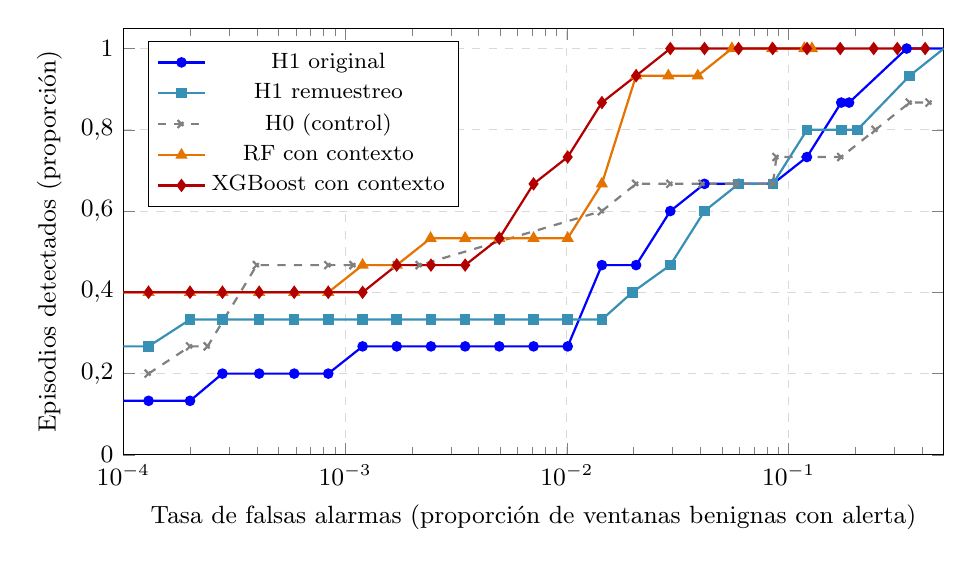
\begin{tikzpicture}
\begin{semilogxaxis}[
    width=12cm, height=7cm,
    xmin=0.0001, xmax=0.5, ymin=0, ymax=1.05,
    xlabel={Tasa de falsas alarmas (proporción de ventanas benignas con alerta)},
    ylabel={Episodios detectados (proporción)},
    grid=major, grid style={dashed,gray!30},
    tick label style={font=\small}, label style={font=\small},
    legend pos=north west, legend style={font=\footnotesize},
    /pgf/number format/use comma,
]
\addplot[thick, blue, mark=*, mark size=1.5pt] coordinates {(0.00009,0.133) (0.00013,0.133) (0.00020,0.133) (0.00028,0.200) (0.00041,0.200) (0.00059,0.200) (0.00084,0.200) (0.00120,0.267) (0.00171,0.267) (0.00244,0.267) (0.00348,0.267) (0.00496,0.267) (0.00708,0.267) (0.01009,0.267) (0.01439,0.467) (0.02053,0.467) (0.02928,0.600) (0.04176,0.667) (0.05957,0.667) (0.08494,0.667) (0.12094,0.733) (0.17270,0.867) (0.18741,0.867) (0.34071,1.000) (0.50117,1.000)};
\addlegendentry{H1 original}
\addplot[thick, cyan!70!black, mark=square*, mark size=1.5pt] coordinates {(0.00009,0.267) (0.00013,0.267) (0.00020,0.333) (0.00028,0.333) (0.00041,0.333) (0.00059,0.333) (0.00084,0.333) (0.00120,0.333) (0.00171,0.333) (0.00244,0.333) (0.00348,0.333) (0.00496,0.333) (0.00708,0.333) (0.01009,0.333) (0.01439,0.333) (0.01974,0.400) (0.02928,0.467) (0.04176,0.600) (0.05957,0.667) (0.08494,0.667) (0.12114,0.800) (0.17278,0.800) (0.20425,0.800) (0.35142,0.933) (0.50117,1.000)};
\addlegendentry{H1 remuestreo}
\addplot[thick, gray, dashed, mark=x, mark size=2pt] coordinates {(0.00013,0.200) (0.00020,0.267) (0.00024,0.267) (0.00040,0.467) (0.00084,0.467) (0.00109,0.467) (0.00171,0.467) (0.00217,0.467) (0.01439,0.600) (0.02052,0.667) (0.02928,0.667) (0.04088,0.667) (0.05859,0.667) (0.08494,0.667) (0.08813,0.733) (0.17259,0.733) (0.24631,0.800) (0.35142,0.867) (0.43172,0.867)};
\addlegendentry{H0 (control)}
\addplot[thick, orange!90!black, mark=triangle*, mark size=1.8pt] coordinates {(0.00009,0.400) (0.00013,0.400) (0.00020,0.400) (0.00028,0.400) (0.00041,0.400) (0.00059,0.400) (0.00084,0.400) (0.00120,0.467) (0.00171,0.467) (0.00243,0.533) (0.00348,0.533) (0.00496,0.533) (0.00708,0.533) (0.01009,0.533) (0.01439,0.667) (0.02052,0.933) (0.02869,0.933) (0.03895,0.933) (0.05549,1.000) (0.08423,1.000) (0.11769,1.000) (0.12739,1.000)};
\addlegendentry{RF con contexto}
\addplot[thick, red!70!black, mark=diamond*, mark size=1.8pt] coordinates {(0.00009,0.400) (0.00013,0.400) (0.00020,0.400) (0.00028,0.400) (0.00041,0.400) (0.00059,0.400) (0.00084,0.400) (0.00120,0.400) (0.00171,0.467) (0.00244,0.467) (0.00348,0.467) (0.00496,0.533) (0.00708,0.667) (0.01009,0.733) (0.01439,0.867) (0.02053,0.933) (0.02928,1.000) (0.04175,1.000) (0.05947,1.000) (0.08474,1.000) (0.12105,1.000) (0.17087,1.000) (0.24187,1.000) (0.30911,1.000) (0.41252,1.000)};
\addlegendentry{XGBoost con contexto}
\end{semilogxaxis}
\end{tikzpicture}
\caption[Episodios detectados frente a la tasa de falsas alarmas en Unraveled.]{Episodios detectados frente a la tasa de falsas alarmas en la partición de prueba de Unraveled, al variar el umbral $\tau$. Los modelos de referencia usan atributos continuos y datos originales. Fuente: Elaboración propia.}
\label{fig:curva_ttd_fpr}
\end{figure}
\FloatBarrier

El umbral calibrado en validación no conserva la tasa de falsas alarmas objetivo en la partición de prueba. En Unraveled, el umbral calibrado para un 0,1~\% produce un 0,75~\% de falsas alarmas en el HMM supervisado y entre 0,5~\% y 1,6~\% en los modelos de referencia, y en DAPT2020 el umbral calibrado para un 1~\% produce un 1,6~\% en el HMM. Por ello, las comparaciones de este capítulo se basan en la curva y no en el punto de operación calibrado.

La tasa de detección previa a la exfiltración resultó nula en todas las configuraciones, pero este valor no refleja el desempeño de los modelos. De los seis episodios de prueba de Unraveled que contienen exfiltración, cinco comienzan directamente con ella, y en DAPT2020 ocurre lo mismo con los dos episodios que la contienen. En esos casos no existe un instante anterior a la exfiltración dentro del episodio en que se pueda emitir una alerta. Esto se debe a que, en Unraveled, cada host cumple casi siempre un único papel en la campaña, de modo que la progresión entre etapas se observa en la red completa y no dentro de la secuencia de un mismo host.

\subsection{Sensibilidad de la configuración}
\label{sec:res_sensibilidad}
Para evaluar las decisiones de preprocesamiento sin recurrir a la partición de prueba, se repitieron las configuraciones del HMM sobre Unraveled variando un aspecto a la vez y evaluando en la partición de validación. La Tabla~\ref{tab:sensibilidad} presenta los resultados de H1 con datos originales. En todas las variantes, el umbral se calibra sobre la misma partición evaluada, por lo que la tasa de falsas alarmas se mantiene en torno al 0,1~\% y las métricas de detección son comparables entre filas.

\begin{table}[h!]
\centering
\small
\renewcommand{\arraystretch}{1.25}
\begin{tabular}{|l|c|c|c|c|c|c|c|c|}
\hline
\textbf{Variante} & $\boldsymbol{M}$ & \textbf{Rec.} & \textbf{Foot.} & \textbf{Lat.} & \textbf{Exf.} & \textbf{Macro} & \textbf{Detec.} & \textbf{TTD} \\ \hline
Base ($\Delta t$ = 5 min, p50 y p95) & 82 & 0,000 & 0,937 & 0,377 & 0,911 & 0,556 & 2/7 & 30 \\ \hline
$\Delta t$ = 1 min & 82 & 0,000 & 0,882 & 0,762 & 0,942 & 0,646 & 3/7 & 9 \\ \hline
$\Delta t$ = 15 min & 82 & 0,000 & 0,639 & 0,422 & 0,372 & 0,358 & 3/7 & 60 \\ \hline
Terciles & 82 & 0,000 & 0,936 & 0,531 & 0,987 & 0,613 & 3/7 & 15 \\ \hline
Solo p95 & 17 & 0,000 & 0,727 & 0,212 & 0,093 & 0,258 & 3/7 & 895 \\ \hline
Encubrimiento excluido & 82 & 0,000 & 0,937 & 0,377 & 0,911 & 0,556 & 2/7 & 30 \\ \hline
\end{tabular}
\caption[Sensibilidad de la configuración del HMM en la partición de validación de Unraveled.]{Sensibilidad de la configuración del HMM (H1 con datos originales) en la partición de validación de Unraveled. $M$: tamaño del alfabeto. Demás columnas como en la Tabla~\ref{tab:res_unraveled}. Fuente: Elaboración propia.}
\label{tab:sensibilidad}
\end{table}
\FloatBarrier

La ventana de un minuto obtiene el mayor $F_1$-score macro, principalmente porque duplica el $F_1$-score del movimiento lateral, y reduce la mediana del tiempo hasta la detección de 30 a 9 minutos. Parte de esta reducción se explica porque una ventana más corta disminuye también la resolución mínima del tiempo hasta la detección. Su costo es computacional: genera cinco veces más ventanas, y su ejecución tomó 43 minutos frente a menos de 10 en las otras sensibilidades. La ventana de quince minutos empeora el desempeño en el \textit{foothold} y en la exfiltración.

En la discretización, los terciles superan a los cortes en los percentiles 50 y 95, con un $F_1$-score macro de 0,613. Este resultado contradice lo que se esperaba al diseñar la discretización, que con terciles casi todas las ventanas de ataque cayeran en el mismo nivel. Usar solo el corte en el percentil 95 reduce el alfabeto a 17 símbolos y degrada el desempeño en el \textit{foothold}, el movimiento lateral y la exfiltración.

La exclusión del encubrimiento produce exactamente los mismos resultados que la configuración base, porque en Unraveled el encubrimiento ocurre solo en la partición de prueba. Esta decisión no puede evaluarse en validación y se contrastará en la validación cruzada por día.

En todas las variantes, el refinamiento con Baum-Welch volvió a ser descartado por la verificación posterior, y el reconocimiento no fue identificado. En cambio, la exfiltración se identifica en validación con un $F_1$-score de 0,911 en la configuración base, mientras que en prueba no se identifica (Tabla~\ref{tab:res_unraveled}). Esta diferencia indica que el comportamiento de la exfiltración cambia entre ambos periodos. Como cada variante se evaluó por separado y la partición de validación contiene solo siete episodios, estos resultados orientan la configuración que se congelará para la evaluación definitiva, pero aún no la determinan. En particular, falta evaluar la combinación de una ventana de un minuto con la discretización por terciles.

\section{Análisis}
\label{sec:analisis_preliminar}
Respecto de las hipótesis de trabajo planteadas en el diseño experimental, los resultados preliminares no respaldan por ahora la primera: a igual tasa de falsas alarmas, el HMM no detecta las campañas antes ni con mayor frecuencia que los modelos de referencia. La segunda hipótesis sí se observa, ya que los modelos de referencia alcanzan un $F_1$-score por ventana superior al del HMM en ambos conjuntos. Los resultados sí confirman dos decisiones del diseño: la estimación supervisada mantiene la correspondencia entre estados y etapas que el entrenamiento no supervisado pierde, y la verificación posterior impide que el refinamiento con Baum-Welch degrade esa correspondencia.

Los resultados también identifican los siguientes aspectos del diseño que requieren ajuste:
\begin{enumerate}
    \item \textbf{Nivel de la secuencia.} Como cada host de Unraveled cumple casi siempre un solo papel, la estructura de transiciones del HMM tiene poca progresión que modelar dentro de una secuencia. Se evaluará combinar las probabilidades filtradas de todos los hosts en una línea de tiempo de la campaña a nivel de red, en la que la progresión entre etapas sí es observable y la detección previa a la exfiltración puede medirse.
    \item \textbf{Observables de la exfiltración.} Ningún modelo identifica la exfiltración de prueba en Unraveled con los cuatro atributos actuales, aunque el HMM sí la identifica en validación. Se analizará qué cambia en el tráfico de exfiltración entre ambos periodos y se evaluará incorporar un atributo que acumule el volumen saliente de un host a lo largo de varias ventanas.
    \item \textbf{Calibración del umbral.} La tasa de falsas alarmas en prueba supera varias veces la objetivo. Se evaluará calibrar el umbral con más días de validación y reportar las métricas de detección siempre junto con la curva completa.
    \item \textbf{Configuración del preprocesamiento.} En validación, la ventana de un minuto y la discretización por terciles superaron a la configuración base. Se evaluará su combinación antes de congelar la configuración.
    \item \textbf{Robustez de la estimación.} Con 15 episodios en Unraveled y 8 en DAPT2020, un episodio cambia la tasa de detección en 6,7 y 12,5 puntos porcentuales, respectivamente. La validación cruzada agrupada por día y el análisis separado por grupo atacante, previstos en el plan, permitirán estimar la variabilidad de estos resultados.
\end{enumerate}

Estos resultados se obtuvieron sobre la partición de prueba con fines exploratorios. Las decisiones de configuración que se tomen a partir de ellos se basarán en la partición de validación, y la evaluación definitiva en prueba se realizará una sola vez, con la configuración congelada.
